  \chapter{Desenvolvimento do chatbot}
  
-  \section{Motivação}
  
  \subsection{Contexto: o projeto PIPA UFRJ}
  
  O Projeto Infância e Poluentes Ambientais – PIPA UFRJ é um estudo epidemiológico denominado "Estudo longitudinal dos efeitos da exposição a poluentes ambientais sobre a saúde infantil - Coorte dos bebês". Este estudo tem como proposta fornecer informação que permita a investigação e análise dos efeitos dos poluentes ambientais especificamente: metais (chumbo, mercúrio, cádmio e arsênio), agrotóxicos e plastificantes, sobre o desenvolvimento das crianças, desde o período de gestação e nascimento, até os 4 anos de idade. 
  
  Em 2017 iniciou-se a fase de estudo piloto do projeto, avaliando a exposição da mãe e seu filho até os 6 meses de idade, além de suas informações sociodemográficas. Nessa fase as metodologias e estratégias propostas estão sendo testadas e validadas, a fim de aprimorar o estudo. Como resultado desse projeto, vai ser possível propor medidas preventivas e de controle, o que melhoraria a qualidade de vida da população.
  
  O projeto é promovido pela Universidade Federal do Rio de Janeiro (UFRJ) realizado pela Maternidade Escola, pela Faculdade de Medicina e pelo Instituto de Estudos em Saúde Coletiva (IESC/UFRJ) e conta com diversos parceiros como a Fundação Oswaldo Cruz (FIOCRUZ) e o Centro de Estudos da Saúde do Trabalhador e Ecologia Humana (CESTEH).
  
  \subsection{Tecnologias utilizadas no PIPABOT}
  \subsubsection{Node.JS}
  Node.js é um interpretador de código JavaScript construído sobre a máquina virtual Javascript V8 do Google, cujo foco é executar aplicações baseadas em rede no lado do servidor.
  
  %Historicamente a linguagem JavaScript é conhecida por ser a linguagem padrão executada por \emph{browsers} no lado do cliente mas com a rápida evolução da web nos últimos anos, os motores de execução da linguagem receberam diversas melhorias, tornando viável a execução de códigos que vão além de manipulação de HTML.
  
  A principal característica que diferencia o Node.js de outras tecnologias \emph{server-side} como o PHP, é o fato de sua execução ser \emph{single-thread}, ou seja, apenas uma thread é responsável por executar a aplicação, enquanto que outras linguagens a execução é \emph{multi-thread}.
  
  Os modelos tradicionais de aplicações web criam novas threads para cada requisição recebida, o que demanda recursos computacionais como memória RAM, por exemplo. Como esses recursos são limitados, haverá um número máximo de threads que poderão ser criadas até que os recursos sejam liberados novamente.
  
  \begin{figure}[h!]
  	\begin{center}
  		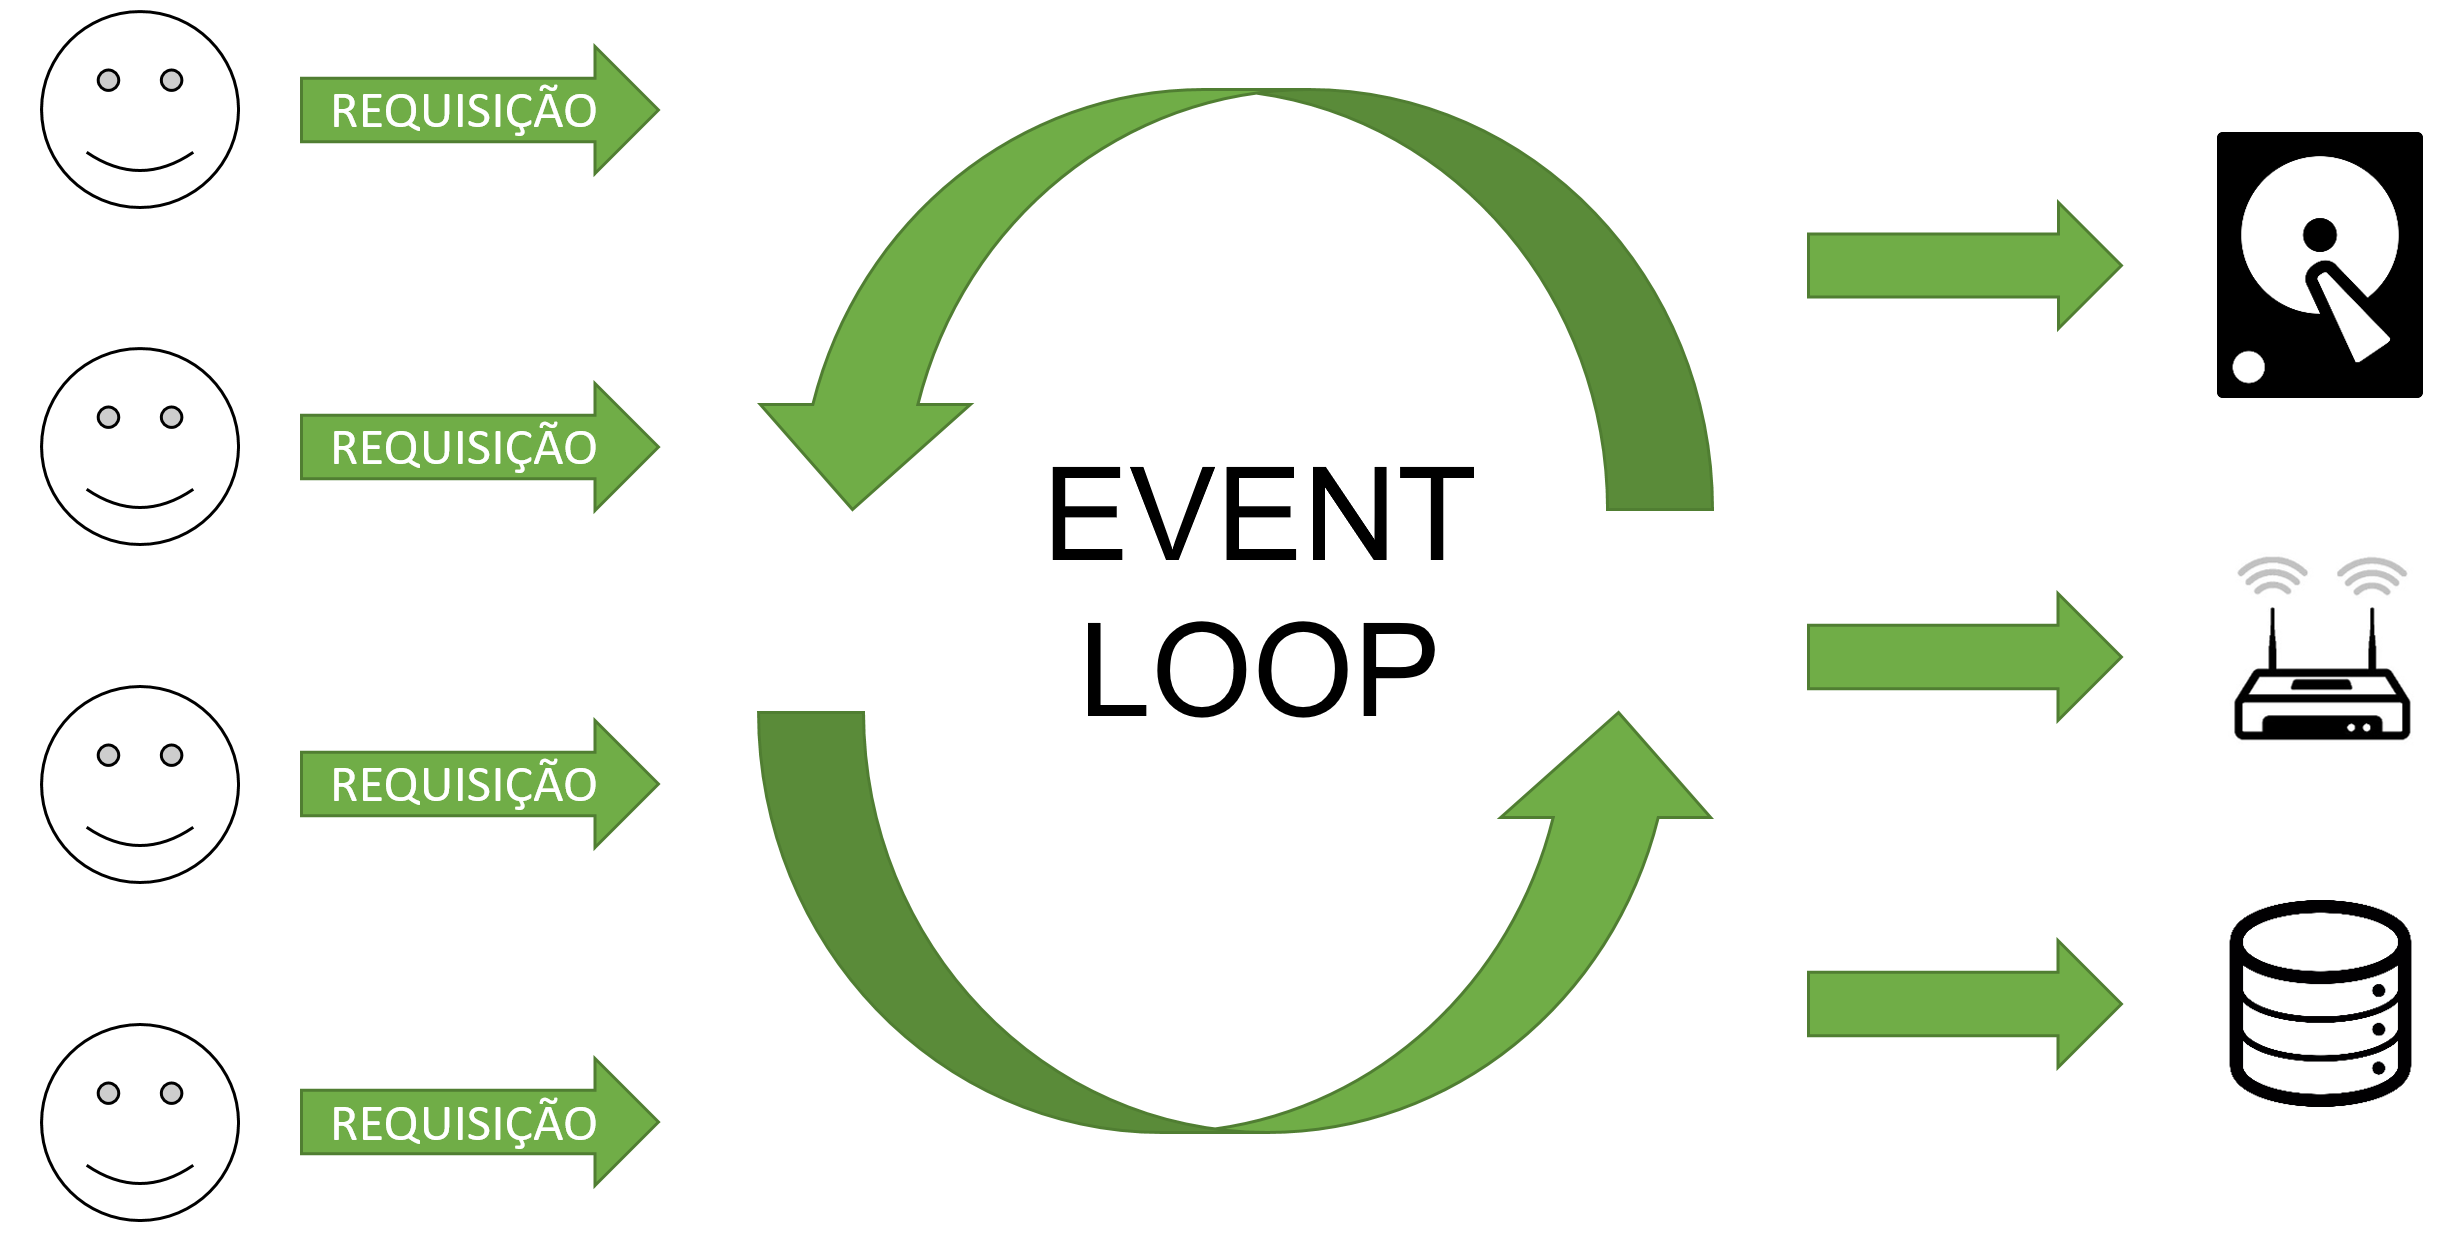
\includegraphics[width=1\linewidth]{images/node_thread.png}
  		\caption{Arquitetura do NodeJS}
  		\label{fig:node}
  	\end{center}
  \end{figure}
    
  No Node.js as requisições são tratadas por uma única thread, chamada de Event Loop. A thread é executada esperando eventos para tratar. Quando chega uma nova requisição, um evento é criado.
  
  Para tratar a concorrência de requisições, o Node.js faz uso de chamadas de E/S não-bloqueantes. Assim, a sua única thread não fica esperando as demais chamadas já realizadas serem concluídas para continuar sua execução.
  
  Graças a sua arquitetura, o Node.js consegue tratar um número maior de requisições concorrentes do que uma aplicação no modelo tradicional, se mostrando como uma das plataformas mais escaláveis da atualidade.
  
  \subsubsection{NPM}
  Node Package Manager, ou NPM, é o gerenciador de pacotes do Node.js. Nele é possível encontrar componentes open-source que agilizam o desenvolvimento de aplicações como conectores para bancos de dados, servidores web completos, entre outros. Além disso, o NPM também faz o gerenciamento de dependências de um projeto.
  
  Ao instalar um componente com o comando \emph{npm install <componente>} em um projeto do Node.js, o utilitário adiciona o pacote e a versão utilizada e suas dependências em um arquivo chamado package.json;  
  Desse modo é possível restaurar todas as dependências do projeto, caso seja necessário.
  
  \subsubsection{Git}
  Git é um sistema de versionamento de código distribuído que possui diversas ferramentas úteis para o desenvolvimento de um sistema. Sua escolha se deu pelo fato de ser open source, e por permitir criar ramificações (branches) de código a partir de um ponto do desenvolvimento, permitindo criar diferentes versões independentes entre os ramos\footnote{https://git-scm.com/about}. Através do uso de branches, foi criado um Git Flow para o PipaBot, como na figura \ref{fig:gitflow}.
  
  \begin{figure}[h!]
  	\begin{center}
  		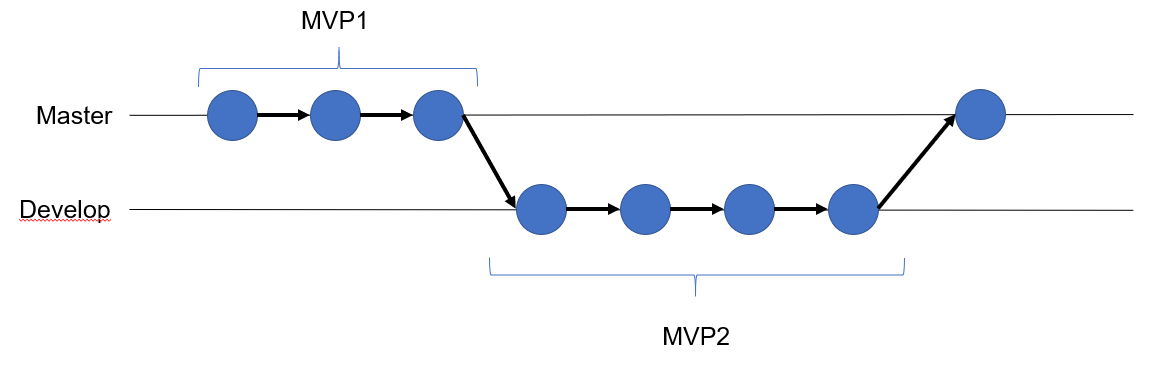
\includegraphics[width=1\linewidth]{images/git_flow.png}
  		\caption{PipaBot - Organização do versionamento do código}
  		\label{fig:gitflow}
  	\end{center}
  \end{figure}
  
  Após o desenvolvimento da primeira versão do PipaBot, foi criada uma nova branch de desenvolvimento da próxima interação do ciclo Construir-Medir-Aprender. Isso foi feito para que a branch principal do repositório (master) possuísse um produto pronto para ser executado. Ao término da segunda versão do MVP, foi feito um merge da branch de desenvolvimento com a master.
  
  

  \section{Ambientes de desenvolvimento} % trocar a ordem com arquitetura?
  O PipaBot foi desenvolvido em uma estrutura formada por dois ambientes: um ambiente de desenvolvimento e um ambiente de homologação.
  
  O ambiente de desenvolvimento é executado no próprio computador onde as implementações são feitas e é acessível apenas localmente. É composto de um servidor HTTP do Botpress, que gera uma instância do PipaBot, tornando possível testar funcionalidades através de um chat na URL \url{http://localhost:3000/s/chat}.
  
  O ambiente de homologação é composto por dois servidores HTTP e um servidor de banco de dados MySQL, todos localizados na nuvem e recebem as versões incrementais do \textit{bot} a cada ajuste funcional, para que sejam testadas e validadas pelos \textit{stakeholders}.
  
  Um dos servidores HTTP é o Botpress, contendo a última release do ambiente de desenvolvimento. O outro servidor HTTP executa uma instância do Wordpress, para que seja permitido simular o Portal do PIPA e validar a versão web do PipaBot. O servidor MySQL é utilizado pelo Wordpress para armazenar os dados dos usuários.
  
  \section{A solução}
  
  \subsection{Arquitetura}
  A arquitetura do PipaBot é composta por duas camadas, o \textit{front-end} e o \textit{back-end}. O \textit{front-end} é toda a interface utilizada pelo usuário para interagir com o bot (comumente chamado de canais): o portal do PIPA através da versão web, ou pelo aplicativo do Messenger em dispositivos mobile ou PC. Enquanto o \textit{back-end} é onde se encontra o processamento do \textit{bot}. É nele onde as mensagens são classificadas e as respostas, escolhidas. Além disso, o back-end também é responsável pela integração dos dados dos pacientes do Portal do PIPA com o \textit{bot}. O esquema detalhado da arquitetura pode ser visto na figura \ref{fig:arquitetura}.
  
	  \begin{figure}[h!]
	  	\begin{center}
		  	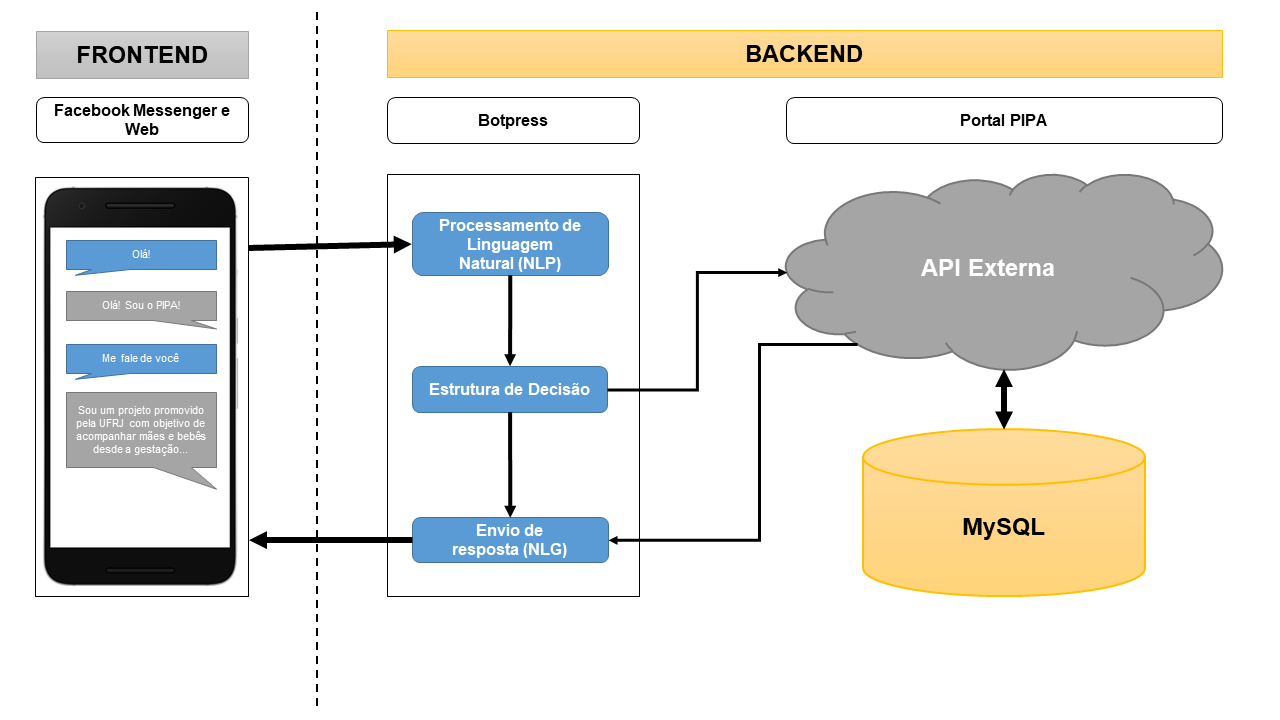
\includegraphics[width=1\linewidth]{images/arquitetura-pipabot.png}
			\caption{Arquitetura do PipaBot}
			\label{fig:arquitetura}
	  	\end{center}
	  \end{figure}
  
  Como framework de criação de bots, foi escolhido o \textbf{\textit{Botpress}}, por possuir, em uma única solução, funções como processamento de linguagem natural, criador de fluxos de conversa, estruturas de decisão (permitindo a criação de chatbots baseados em regras ou em inteligência artificial, através de classificação de intents) e suportar diversos canais de comunicação para um mesmo \textit{bot}, além de ser uma estrutura onde todo o código fica sob domínio do administrador do \textit{bot}, o que é importante principalmente para implementações de funcionalidades específicas do \textit{PipaBot} como o acesso à base de usuários, por exemplo.
  
  Para integrar o PipaBot ao Portal do PIPA, que é desenvolvido utilizando o sistema de gestão de conteúdo Wordpress (construído em PHP e MySQL), foi utilizada a própria API REST do Wordpress. Essa API implementa endpoints que permitem acessar o CRUD (\textit{Create}, \textit{Read}, \textit{Update} e \textit{Delete} - Operações de leitura e escrita de dados do sistema) de diversas tabelas que guardam o conteúdo do Portal no banco de dados, inclusive de usuários. Contudo, por padrão, as rotas de leitura de usuários apenas retornam usuários que já fizeram alguma publicação no Portal, o que não era o caso dos pacientes, que nem possuem permissão de executar tal ação. Então, foram criados três novos \textit{endpoints}, que só podem ser acessado através de autenticação através da tecnologia JWT (\textit{JSON Web Token}), que utiliza o perfil de um usuário administrador do Portal. Esses \textit{endpoints} são responsáveis por (I) verificar se um usuário existe através do seu CPF e ano de nascimento, e (II) por adicionar um identificador do usuário do \textit{chatbot} no cadastro do Portal e (III) por verificar se um usuário do bot está atrelado a um cadastro de paciente no Portal - através do identificador cadastrado no \textit{endpoint} II. 
  
  Para tornar a instalação dos recursos do PipaBot mais ágil e manutenível, todos as implementações dos \textit{endpoints} foram encapsulados em um arquivo PHP que é reconhecido pela instalação do Wordpress como um plugin, que pode ser ativado ou desativado a qualquer momento através do painel do administrativo do Portal.
  
  \subsection{Modelos}
  	\begin{center}
  		\begin{tabular}{ | m{0.2\linewidth} | m{0.26\linewidth} | m{0.26\linewidth} | m{0.26\linewidth} | } 
  			\hline
  			\textbf{Identificação} & \multicolumn{3}{l|}{RF01}\\ 
  			\hline
  			\textbf{Casos de Uso Relacionados} & \multicolumn{3}{l|}{TESTE}\\ 
  			\hline
  			\textbf{Descrição} & \multicolumn{3}{l|}{Lorem ipsum damet...}\\ 
  			\hline
  			\textbf{Prioridade} & [ ] Essencial & [ ] Importante & [ ] Desejável \\
  			\hline
  		\end{tabular}
  	\end{center}
  
%	-  	Mapeamento de casos de uso
	
%	-	Diagrama de Atividades
	
%	-	Especificação dos Requisitos
	\begin{figure}[h!]
	 	\begin{center}
	 		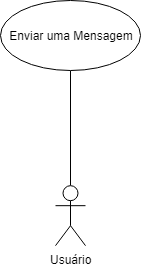
\includegraphics[scale=0.6]{images/UC_Usuario.png}
	 		\caption{Casos de Uso do Usuário}
	 		\label{fig:ucusuario}
	 	\end{center}
	\end{figure}

	\begin{figure}[h!]
		\begin{center}
			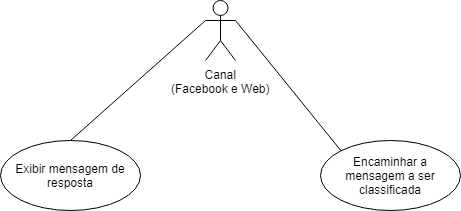
\includegraphics[width=12cm]{images/UC_Canal.png}
			\caption{Casos de Uso do Canal (Messenger e Web)}
			\label{fig:uccanal}
		\end{center}
	\end{figure}
	
	\begin{figure}[h!]
		\begin{center}
			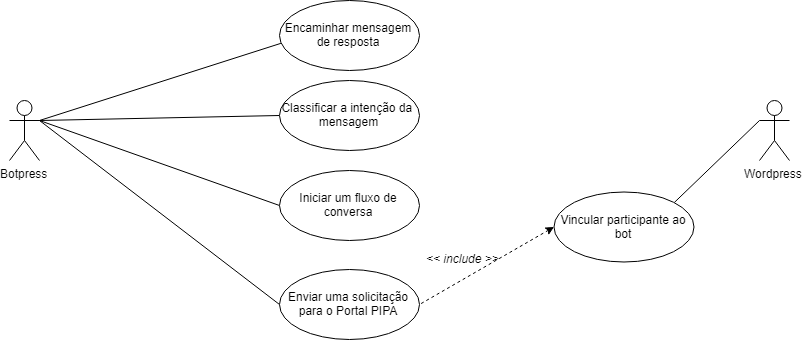
\includegraphics[width=1\linewidth]{images/UC_Botpress_Wordpress.png}
			\caption{Casos de Uso do Bot}
			\label{fig:ucbot}
		\end{center}
	\end{figure}
  \FloatBarrier
  \subsection{MVP 1}
  Tendo como principal problema a falta de engajamento das mães com o projeto e buscando criar um novo canal de informação sobre o PIPA, o PipaBot teve a sua primeira versão orientada a regras. Para garantir que o usuário navegasse através dos fluxos de conversa, o \textit{bot} exibia botões, de modo que o usuário não desviasse a conversa para um outro assunto no meio de um fluxo. Essa versão era capaz de dar informações sobre o funcionamento e objetivo do projeto, e vincular usuários a um cadastro no Portal do PIPA.
  
  O principal objetivo da primeira versão era apresentar aos pesquisadores do projeto o que um \textit{chatbot} poderia ser capaz de fazer, demonstrando integrações com o sistema do PIPA e elementos de interação, visando novas ideias para a versão seguinte.
  \subsection{MVP 2}
  A segunda versão do PipaBot trouxe diversas melhorias. Foram criados diálogos exclusivos para pacientes do projeto como informações sobre consultas e exames além de ter também o treinamento para diversos \textit{intents}, que eram reconhecidos através da tecnologia de NLP do Botpress. Cada \textit{intent} levava a um fluxo de conversa diferente cuja interação poderia ser feita não somente por botões, mas textualmente, dando mais naturalidade ao diálogo.
  \subsection{Avaliação do produto}
  %falar do TAM e mostrar os resultados. 
  Para avaliar o PipaBot foi utilizado o modelo TAM (\textit{Technology Acceptance Model})\cite{tam_davis} que procura determinar os aspectos de utilidade e facilidade de uso de tecnologias. Para isso, o TAM se baseia nos conceitos de \textbf{percepção de utilidade} e \textbf{percepção de facilidade de uso}, métricas que avaliam, respectivamente, o quanto o usuário acredita que a tecnologia possa melhorar seu desempenho e o quanto ele acredita que, ao utilizar a tecnologia, ele possa ficar livre de esforço físico e mental.
  
  Para elaboração do TAM, foi utilizado o paradigma GQM (\textit{Goal/Question/Metric}), ilustrado na figura \ref{fig:gqm}, que consiste em descrever os objetivos (\textit{Goals}), a partir dos objetivos elaborar um conjunto de questões (\textit{Questions}) e, então, métricas (\textit{metrics}) para medir as respostas. Os objetivos do PipaBot estão definidos nas tabelas abaixo.
  
  \begin{figure}[h!]
  	\begin{center}
  		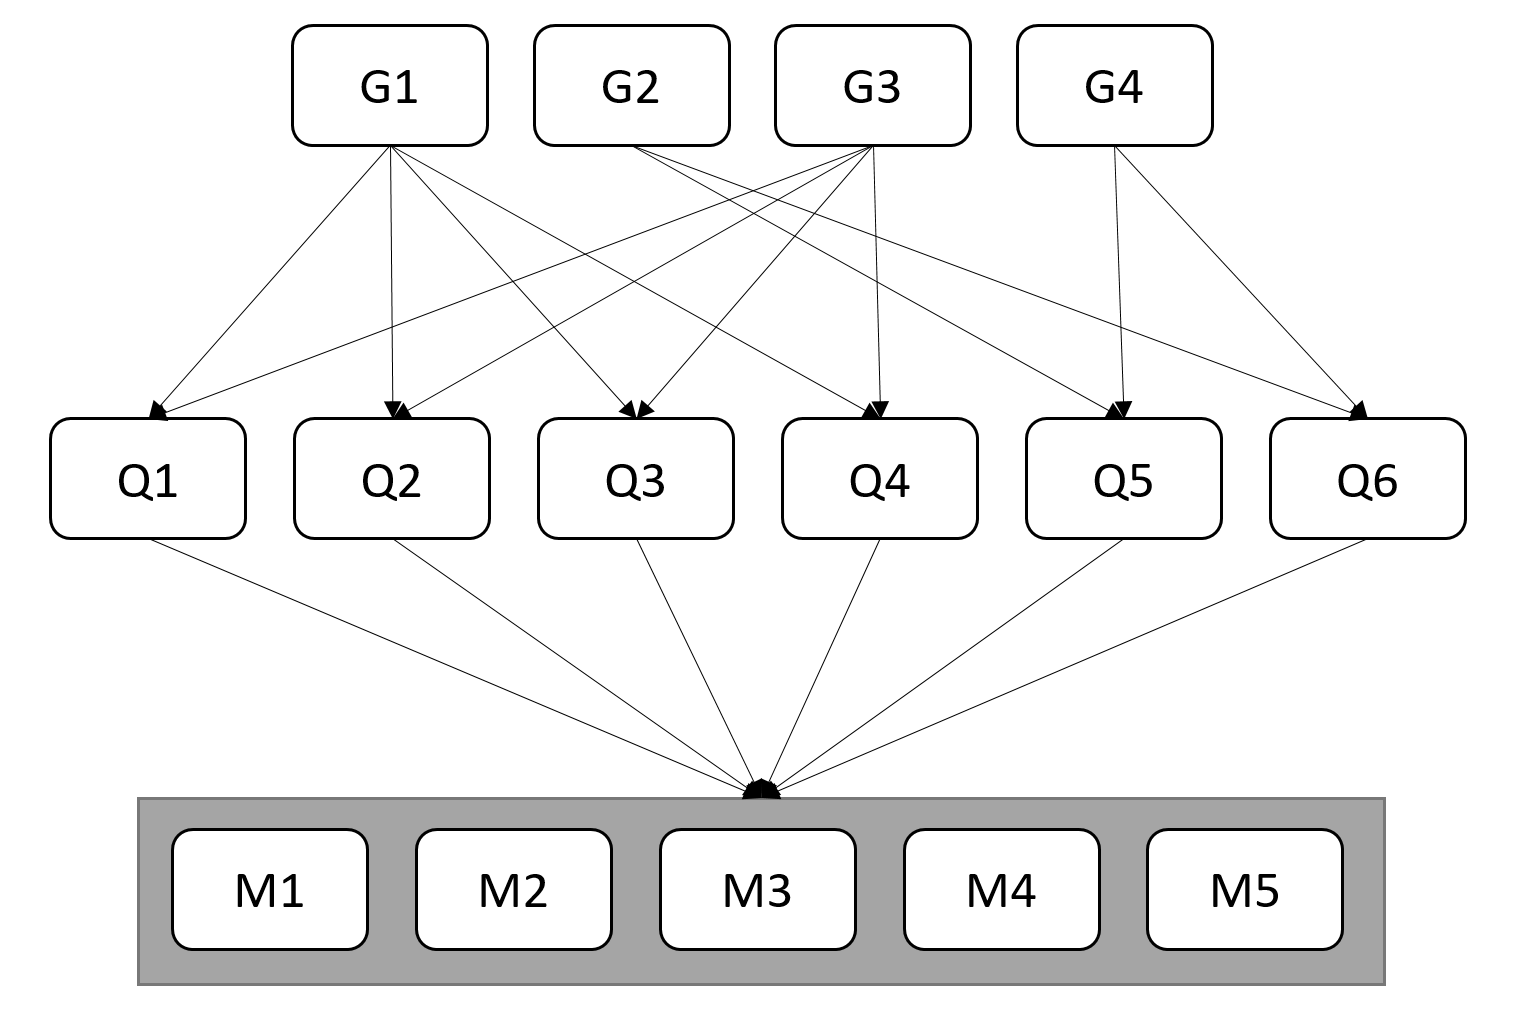
\includegraphics[width=1\linewidth]{images/gqm.png}
  		\caption{Organização do Paradigma GQM aplicado ao PipaBot}
  		\label{fig:gqm}
  	\end{center}
  \end{figure}
  
  \begin{center}
  	\begin{table}[h!]
  		\begin{tabular}{ | m{0.35\linewidth} | m{0.65\linewidth} | } 
  			\hline
  			\textbf{Analisar} & O PipaBot (chatbot do PIPA) \\ 
  			\hline
  			\textbf{Com o propósito de} & Caracterizar \\ 
  			\hline
  			\textbf{Com respeito a} & Facilidade de uso (número de mensagens e tempo de resposta) \\ 
  			\hline
  			\textbf{Sob o ponto de vista de} & Profissionais de computação \\
  			\hline
  			\textbf{No contexto de} & Profissionais de computação (estudantes de graduação e pós graduação) realizando tarefas de busca de informação no PipaBot. \\
  			\hline
  		\end{tabular}
  	  \caption{GQM - Objetivo 1}
  	  \label{tab:obj1}  	  
  	\end{table}
  \end{center}

	\begin{center}
		\begin{table}[h!]
			\begin{tabular}{ | m{0.35\linewidth} | m{0.65\linewidth} | } 
				\hline
				\textbf{Analisar} & O PipaBot (chatbot do PIPA) \\ 
				\hline
				\textbf{Com o propósito de} & Compreender \\ 
				\hline
				\textbf{Com respeito a} & Utilidade (pertinência e adequação do conteúdo da resposta) \\ 
				\hline
				\textbf{Sob o ponto de vista de} & Profissionais de computação \\
				\hline
				\textbf{No contexto de} & Estudantes de graduação e pós-graduação do sexo feminino realizando tarefas de busca de informação no PipaBot. \\
				\hline
			\end{tabular}
			\caption{GQM - Objetivo 2}
			\label{tab:obj2}
		\end{table}
	\end{center}
	
	\begin{center}
		\begin{table}[h!]
			\begin{tabular}{ | m{0.35\linewidth} | m{0.65\linewidth} | } 
				\hline
				\textbf{Analisar} & O PipaBot (chatbot do PIPA) \\ 
				\hline
				\textbf{Com o propósito de} & Caracterizar \\ 
				\hline
				\textbf{Com respeito a} & Facilidade de uso (número de mensagens e tempo de resposta) \\ 
				\hline
				\textbf{Sob o ponto de vista de} & Profissionais de saúde \\
				\hline
				\textbf{No contexto de} & Profissionais de saúde (estudantes de pós-graduação) realizando tarefas de busca de informação no PipaBot. \\
				\hline
			\end{tabular}
			\caption{GQM - Objetivo 3}
			\label{tab:obj3}
		\end{table}
	\end{center}

	\begin{center}
		\begin{table}[h!]
			\begin{tabular}{ | m{0.35\linewidth} | m{0.65\linewidth} | } 
				\hline
				\textbf{Analisar} & O PipaBot (chatbot do PIPA) \\ 
				\hline
				\textbf{Com o propósito de} & Compreender \\ 
				\hline
				\textbf{Com respeito a} & Utilidade (pertinência, adequação e utilidade do conteúdo da resposta) \\ 
				\hline
				\textbf{Sob o ponto de vista de} & Profissionais de saúde \\
				\hline
				\textbf{No contexto de} & Estudantes do sexo feminino de pós-graduação na área da saúde realizando tarefas de busca de informação no PipaBot. \\
				\hline
			\end{tabular}
			\caption{GQM - Objetivo 4}
			\label{tab:obj4}
		\end{table}
	\end{center}

	Foi elaborado um conjunto de 6 questões abordando os objetivos G1, G2, G3 e G4, visando capturar a percepção de facilidade de uso e utilidade na visão dos usuários. Para medir esses dados foi utilizada a escala \textit{Likert}, no qual os participantes especificam seu nível de concordância com uma afirmação. As questões e métricas estão exibidas nas tabelas \ref{tab:questoes} e \ref{tab:metricas} respectivamente. Junto as métricas foi disponibilizado um espaço para que os participantes pudessem expressar seus comentários sobre cada questão.
	
	\begin{center}
		\begin{table}[h!]
			\centering
			\begin{tabular}{ | m{0.05\linewidth} | m{0.95\linewidth} | } 
				\hline
				\textbf{Q1} & O PipaBot é fácil de usar \\ 
				\hline
				\textbf{Q2} & O PipaBot responde rapidamente aos meus questionamentos \\ 
				\hline
				\textbf{Q3} & Eu posso obter a informação que desejo com poucas perguntas \\ 
				\hline
				\textbf{Q4} & Os elementos de navegação (menus e botões) do PipaBot facilitam a interação ao longo da conversa \\
				\hline
				\textbf{Q5} & O PipaBot fornece respostas pertinentes aos meus questionamentos \\
				\hline
				\textbf{Q6} & O PipaBot fornece respostas adequadas aos meus questionamentos \\
				\hline
			\end{tabular}
			\caption{GQM - Questões para avaliação de grau de concordância}
			\label{tab:questoes}
		\end{table}
	\end{center}

	\begin{center}
		\begin{table}[h!]
			\centering
			\begin{tabular}{ | m{0.05\linewidth} | m{0.3\linewidth} | } 
				\hline
				\textbf{M1} & Concordo Totalmente \\ 
				\hline
				\textbf{M2} & Concordo Parcialmente \\ 
				\hline
				\textbf{M3} & Indiferente \\ 
				\hline
				\textbf{M4} & Discordo Parcialmente \\
				\hline
				\textbf{M5} & Discordo Totalmente \\
				\hline
			\end{tabular}
			\caption{GQM - Métricas}
			\label{tab:metricas}
		\end{table}
	\end{center}

	...

